\begin{frame}{Alcance}

\framesubtitle{Propuesta}
\begin{center}
Reconocer actividades humanas utilizando tel�fonos m�viles modernos
con un enfoque colaborativo
\par\end{center}

\end{frame}
%
\begin{frame}{Alcance}

\framesubtitle{Objetivo General}
\begin{center}
El objetivo principal es desarrollar un sistema \structure{HAR} utilizando
tel�fonos m�viles modernos cuyo aporte principal es una librer�a de
c�digo abierto y un modelo de aprendizaje activo.
\par\end{center}

\end{frame}
%
\begin{frame}{Alcance}

\framesubtitle{Objetivos Espec�ficos}

\setbeamercovered{transparent}
\begin{enumerate}[<+->]
\item Definir el marco te�rico sobre \structure{HAR}. 
\item Revisar las t�cnicas de \structure{captura de se�ales}. 
\item Revisar el \structure{procesamiento de se�ales} para identificar
variables de entrenamiento. 
\item Comprender la clasificaci�n basada \structure{aprendizaje autom�tico}. 
\item Dise�ar un \structure{sistema HAR} que incluya la recolecci�n de
muestras colaborativas y clasificaci�n de actividades en-l�nea. 
\item Aportar un componente de \structure{software libre} para tel�fonos
m�viles modernos con plataforma \emph{\textbf{\emph{Android}}}. 
\end{enumerate}
\end{frame}
%
\begin{frame}{Alcance}

\framesubtitle{Actividades Humanas}

\setbeamercovered{transparent}
\begin{columns}

\column{0.25\textwidth}
\begin{itemize}
\item Acciones cortas

\pause{}
\item Actividades Simples

\pause{}
\item Actividades Complejas
\begin{itemize}
\item Combinaci�n
\item Cotidianas 
\item Gimn�sticas
\item Militares
\end{itemize}

\pause{}
\end{itemize}

\column{0.75\textwidth}
\begin{overprint}
\onslide<1-3> 
\begin{center}
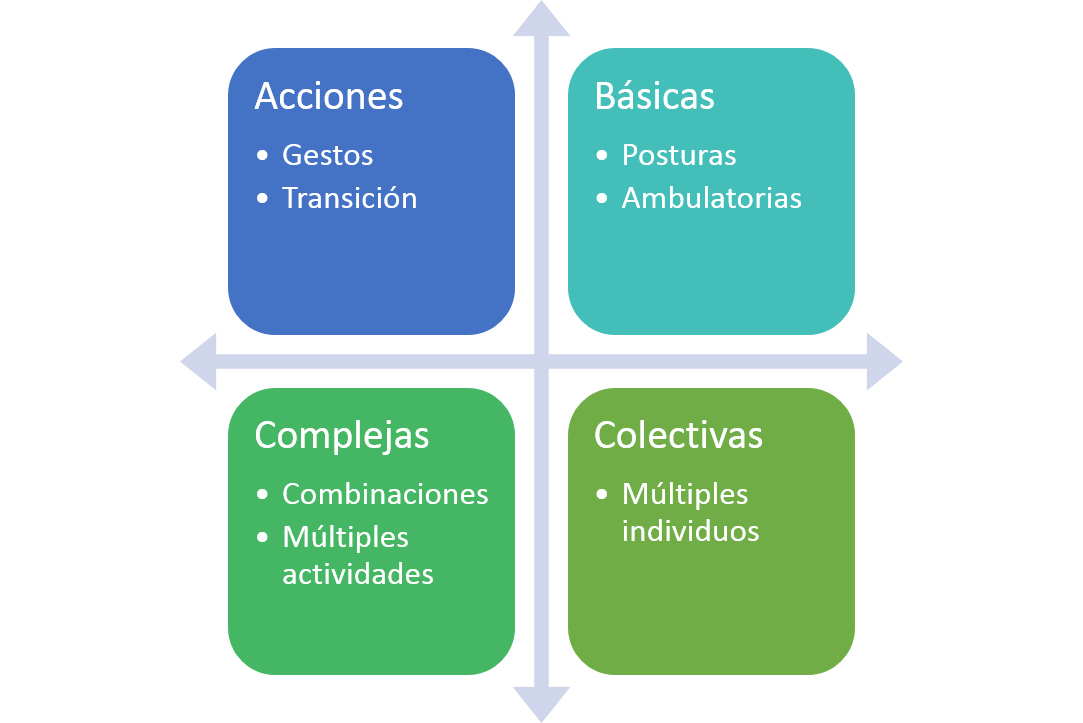
\includegraphics[width=0.95\columnwidth]{propuesta/graphics/actividades}
\par\end{center}
\onslide<4> 
\begin{center}
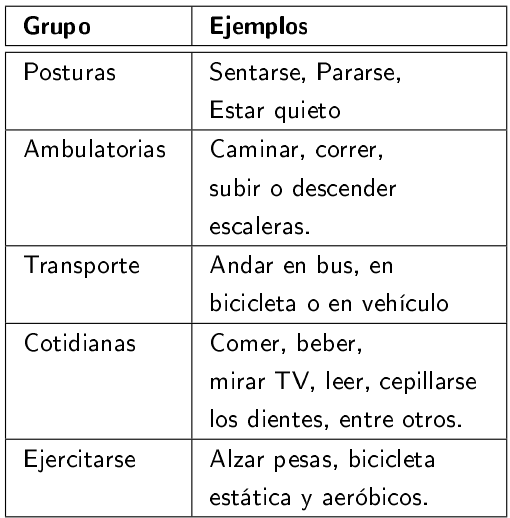
\includegraphics[width=0.7\columnwidth]{intro/graphics/actividades}
\par\end{center}
\end{overprint}
\end{columns}

\end{frame}

